% Introduction chapter.
%
% Developed for my Master Thesis at Maastricht University.
% Based on Eugenio Senes's template at the University of Torino.
%
% By Joeri Hermans (joeri@joerihermans.com)
%
% Released under an MIT license. Share, modify and enjoy, but quote the author!

\chapter{Introduction}
\label{chapter:introduction}

In this chapter we introduce the main concept, and problems surrounding the parallization of gradient descent. We familliarize the reader with the topic and some notation by providing some context why someone would like to apply said technique. Furthermore, in Section~\ref{sec:problem_statement}, we summarize the problem statement and provide several research questions which will guide the research in this work. Finally, we conclude this chapter in Section~\ref{sec:thesis_outline} with a brief outline of the thesis.

\section{Motivation}
\label{sec:motivation}

In recent years it has been shown that being able to train large and deep neural networks result in state-of-the-art performance~\cite{wu2016google, dean2012large}, especially regarding unsupervised feature learning and image recognition. However, consider the required time, and cost of the infrastructure that would be required in order to train a large model in a reasonable amount of time. Furthermore, it is not only the training time and cost of the infrastructure which need to be taken into consideration, but also the volume of the data. The amount of information that will be gathered will be an increasing important factor in the next few years. Not only with respect to big technology companies and government organizations, but also scientific surveys with limited budgets. These scientific surveys will generate more experimental data than ever~\cite{hllhcdesignreport, ivezic2008lsst}, and will have to process and analyze that data. To solve the problem of increased computational workloads and budget freezes, the High Energy Physics (HEP) community is exploring and researching machine learning approaches to fit physics problems~\cite{bian2016recent, de2017learning, louppe2016learning} with the intention to improve detection quality, or reduce computational constraints.\\

However, the sheer size of these datasets severly impacts the training time of the models. In order to resolve this issue, one could sample some representative subset of the data to reduce the training time. The disadvantage of this approach is that some instances, i.e., data points, might not appear in the final training set. This is especially a problem in Deep Learning, where models usually benifit from having access to a lot of training data due to the high dimensionality of the parametrization~\cite{dean2012large}. To resolve this issue, Dean et al.~\cite{dean2012large} introduce two new paradigms to decrease the training time of a large model. The two paradigms, \emph{Model Parallelism}, briefly discussed in Section~\ref{sec:intro_model_parallelism}, and \emph{Data Parallelism}, discussed in Section~\ref{sec:intro_data_parallelism}, are inherently different ways of decreasing the training time of a model.\\

The first paradigm, \emph{Model Parallelism}, is intuitively the most straightforward paradigm since it deals with the parallelization of the computations within a \emph{single} model, i.e., how to parallelize the computations of a single model over multiple machines, or multiple processes. The second paradigm, which will be the main focus of this thesis, is \emph{Data Parallelism}. As stated above, the main concept of data parallelism will be discussed in detail in Section~\ref{sec:intro_data_parallelism}. However, for completion, think of Data Parallelism as a technique to \emph{parallelize gradient descent}. This is done by allocating $n$ processes over possibly $n$ different machines, and splitting the training set into $n$ \emph{partitions}, or \emph{data shards}. For further convenience, we will call such a process a \emph{worker}. In the next step, we assign a single distinct partition to a worker. Meaning, the worker will not be able to fetch training data from other partitions since those have been assigned to different workers. However, in certain data parallel settings, it is benificial to actually consume data from other partitions, once a worker has finished its partition. Finally, the goal of these workers is to work together, and optimize the parameters of a central model.\\

A lot of different distributed optimization schemes have been suggested in recent years~\cite{zhang2015deep, dean2012large, hadjis2016omnivore}. Most of the recent contributions try to push the limits of asynchronous data parallelism, discussed in Section~\ref{sec:asynchronous_data_parallelism}, by simply \emph{annealing} the gradients with respect to some hyperparameter to improve the convergence when the number of workers increases. This suggests that there is an intrinsic limit to asynchronous data parallelism, as suggested by~\cite{implicitmomentum}. As a result, why don't we simply reduce the number of parallel workers if we reduce the impact of the gradient updates by means of annealing anyway? The approach of reducing the number of parallel workers in such a situation has been suggested by~\cite{hadjis2016omnivore}, where they perform a \emph{grid-search} of the training hyperparamers (this includes the number of workers) in order to provide the optimal hyperparameters within a training epoch. However, the disadvantage of this technique is that after every epoch, or a specific number of iterations, a grid-search of the hyperparameters has to be performed in order to obtain the optimal configuration of the hyperparameters to ensure convergence.\\

This brings us to the main motivation behind this work. We intent to obtain a better understanding of \emph{asynchronous} Data Parallism by building upon previous work, and combine it with novel insights to construct a new distributed optimization scheme without introducing new hyperparameters, or relying on grid-searches to optimize the configuration of existing hyperparameters.

\section{Model Parallelism}
\label{sec:intro_model_parallelism}

In \emph{model parallelism}, a single model is distributed over multiple machines~\cite{dean2012large}. The performance benefits of distributing a deep network across multiple machines mainly depends on the structure of the model. Models with a large number of parameters typically benefit from access to more CPU cores and memory, up to the point where communication costs, i.e., propagation of weight updates and synchronization mechanisms, dominate~\cite{dean2012large}.\\

Let us start with a simple example in order to illustrate this concept more clearly. Imagine having a perceptron, as depicted in Figure~\ref{fig:introduction_model_parallelism_perceptron}. In order to parallelize this efficiently, we can view a neural network as a dependency graph, where the goal is to minimize the number of synchronization mechanisms, assuming we have unlimited resources. Furthermore, a synchronization mechanism is only required when a node has more than 1 \emph{variable} dependency. A variable dependency is a dependency which can change in time. For example, a bias would be a \emph{static} dependency, because the value of a bias remains constant over time. In the case for the perceptron shown in Figure~\ref{fig:introduction_model_parallelism_perceptron}, the parallelization is quite straightforward. The only synchronization mechanism which should be implemented resides in output neuron since $y \triangleq \sigma(\sum_i w_ix_i$) where $\sigma$ is the activation function of the output neuron.

\begin{figure}[H]
  \centering
  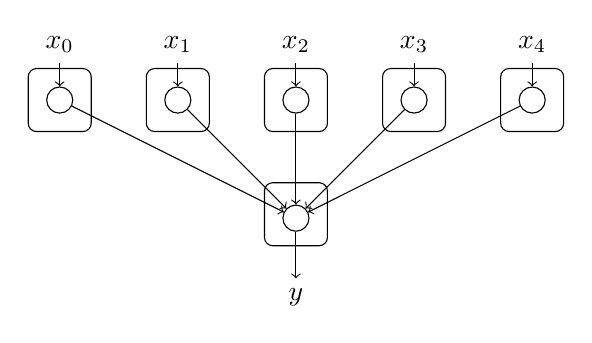
\begin{tikzpicture}

    % Draw inputs.
    \node (i_0) at (-3, 0.7) {$x_0$};
    \node (i_1) at (-1.5, 0.7) {$x_1$};
    \node (i_2) at (0, 0.7) {$x_2$};
    \node (i_3) at (1.5, 0.7) {$x_3$};
    \node (i_4) at (3, 0.7) {$x_4$};


    % Draw the input neurons.
    \node[circle, minimum size=0.2cm, thin, draw=black] (1) at (-3,0) {};
    \node[circle, minimum size=0.2cm, thin, draw=black] (2) at (-1.5,0) {};
    \node[circle, minimum size=0.2cm, thin, draw=black] (3) at (0,0) {};
    \node[circle, minimum size=0.2cm, thin, draw=black] (4) at (1.5,0) {};
    \node[circle, minimum size=0.2cm, thin, draw=black] (5) at (3,0) {};

    % Draw the output neuron.
    \node[circle, minimum size=0.2cm, thin, draw=black] (6) at (0, -1.5) {};

    % Draw output.
    \node (y) at (0, -2.5) {$y$};

    % Draw the lines.
    % X -> Input.
    \draw[->] (i_0) -- (1);
    \draw[->] (i_1) -- (2);
    \draw[->] (i_2) -- (3);
    \draw[->] (i_3) -- (4);
    \draw[->] (i_4) -- (5);
    % Input -> Output.
    \draw[->] (1) -- (6);
    \draw[->] (2) -- (6);
    \draw[->] (3) -- (6);
    \draw[->] (4) -- (6);
    \draw[->] (5) -- (6);
    % Output.
    \draw[->] (6) -- (y);

    % Draw the nodes.
    \draw[rounded corners=3pt] (-3.4,0.4) rectangle ++(0.8,-0.8);
    \draw[rounded corners=3pt] (-1.9,0.4) rectangle ++(0.8,-0.8);
    \draw[rounded corners=3pt] (-0.4,0.4) rectangle ++(0.8,-0.8);
    \draw[rounded corners=3pt] (1.1,0.4) rectangle ++(0.8,-0.8);
    \draw[rounded corners=3pt] (2.6,0.4) rectangle ++(0.8,-0.8);
    \draw[rounded corners=3pt] (-0.4,-1.05) rectangle ++(0.8,-0.8);
  \end{tikzpicture}
  \caption{A perceptron partitioned using the \emph{model parallelism} paradigm. In this approach every input node is responsible for accepting the input $x_i$ from some source, and multiplying the input with the associated weight $w_i$. After the multiplication, the result is sent to the node which is responsible for computing $y$. Of course, this node requires a synchronization mechanism to ensure that the result is consistent. The synchronization mechanism does this by waiting for the results $y$ depends on.}
  \label{fig:introduction_model_parallelism_perceptron}
\end{figure}

\section{Data Parallelism}
\label{sec:intro_data_parallelism}

Data parallelism is an inherently different methodology of optimizing parameters. As stated above, it is a technique to reduce the overall training time of a model. In essence, data parallelism achieves this by having $n$ workers optimizing a central model, and at the same time, processing $n$ different shards (partitions) of the dataset in parallel over multiple workers\footnote{As stated in Section~\ref{sec:motivation}, a worker is a process on a single machine. However, it is possible that multiple workers share the same machine. Nevertheless, one could construct the distribution mechanism (even manually) in such a way every worker will be placed on a different machine.}. The workers are coordinated in such a way that they optimize the parametrization of a central model, which we denote by $\tilde{\theta}_t$. The coordination mechanism of the workers can be implemented in many different ways. Nevertheless, a popular approach to coordinate workers in their task to optimize the central objective, is to employ a centralized \emph{Parameter Server} (PS). The sole responsibility of the parameter server is to aggregate model updates coming from the workers (\emph{worker commits}), and to handle parameter requests (\emph{worker pulls}). In general, there are several approaches towards data parallelism, where some do not require a parameter server. However, all approaches can be categorized into two main groups, i.e., \emph{Synchronous Data Parallelism}, and \emph{Asynchronous Data Parallelism}.\\

\emph{Synchronous Data Parallelism} can be usually identified by the presence of one or multiple locking mechanisms. As in Software Engineering, the purpose of these locking mechanisms is to preserve the consistancy of the state of a model. As an example, let us consider mini-batch parallelism in Figure~\ref{fig:minibatch_data_parallelism} for a moment. Despite it is trivial to implement locally, one could view mini-batch parallelism as an instance of synchronous data parallelism. First and foremost, mini-batch parallelism is a data parallel technique because we split the mini-batch into several partitions where every partition is consumed by its own worker to produce the sum of the gradients, or \emph{accumulated gradient}, as a result. Finally, mini-batch parallelism is synchronous in nature because in order to compute $\theta_{t+1}$, we need to obtain the averaged gradients $\frac{\sum_i \nabla_\theta \mathcal{L}(\theta_t~;~\textbf{x}_i~;~\textbf{y}_i)}{m}$, which is actually the sum of the accumulated gradients of all workers, divided by the number of training instances $m$ in the original mini-batch. As a result, the synchronization barrier is present right before the averaging of the accumulated gradients, since these are the intermediary results we have to wait for before applying a gradient update.

\begin{figure}[H]
  \centering
  % Define database shape.
  \def\database at (#1,#2){
    \draw (#1,#2) ellipse (0.5 and 0.15);
    \draw (#1 - 0.5, #2) -- (#1 - 0.5, #2 - 1);
    \draw (#1 + 0.5, #2) -- (#1 + 0.5, #2 - 1);
    \draw (#1 - 0.5, #2 - 1/3) arc (180:360:0.5 and 0.15);
    \draw (#1 - 0.5, #2 - 2/3) arc (180:360:0.5 and 0.15);
    \draw (#1 - 0.5, #2 - 1) arc (180:360:0.5 and 0.15);
  }
  \def\minibatch at (#1,#2){
    \draw[rounded corners=3pt, draw=black!20, fill=black!10] (#1 - 1.08, #2) rectangle (#1 + 1.08, #2 - 0.8);
    \draw[rounded corners=2pt, draw=blue!35, fill=blue!25, anchor=north] (#1 - 0.25, #2 - 0.4 + 0.25) rectangle (#1 + 0.25, #2 - 0.4 - 0.25);
    \draw[rounded corners=2pt, draw=blue!35, fill=blue!25, anchor=north] (#1 - 0.25 - 0.6, #2 - 0.4 + 0.25) rectangle (#1 + 0.25 - 0.6, #2 - 0.4 - 0.25);
    \draw[rounded corners=2pt, draw=blue!35, fill=blue!25, anchor=north] (#1 - 0.25 + 0.6, #2 - 0.4 + 0.25) rectangle (#1 + 0.25 + 0.6, #2 - 0.4 - 0.25);
    \draw[->] (#1, #2 - 0.9) -- (#1, #2 - 1.5);
  }
  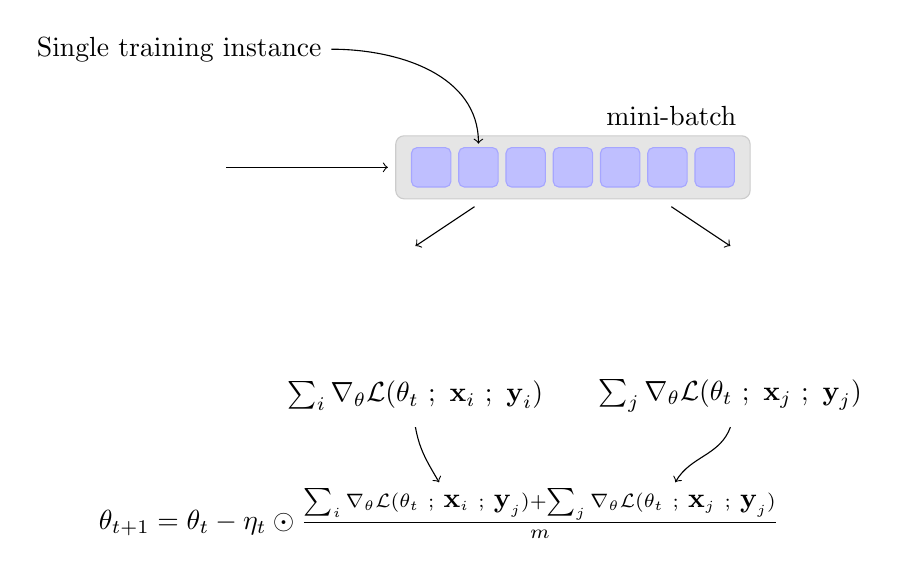
\begin{tikzpicture}
    % Draw the dataset.
    \database at (-5, 0.5);
    \draw[->] (-4.4, 0) -- (-2.35, 0);
    % Draw the minibatch container.
    \draw[rounded corners=3pt, draw=black!20, fill=black!10] (-2.25, 0.4) rectangle (2.25, -0.4);
    % Place the mini-batch label.
    \node at (1.25, 0.65) {mini-batch};
    % Draw the instances inside the minibatch.
    % Center
    \draw[rounded corners=2pt, draw=blue!35, fill=blue!25] (-0.25, 0.25) rectangle (0.25, -0.25);
    % Left
    \draw[rounded corners=2pt, draw=blue!35, fill=blue!25] (-0.25 - 0.6, 0.25) rectangle (0.25 - 0.6, -0.25);
    \draw[rounded corners=2pt, draw=blue!35, fill=blue!25, anchor=north] (-0.25 - 1.2, 0.25) rectangle (0.25 - 1.2, -0.25);
    \draw[rounded corners=2pt, draw=blue!35, fill=blue!25] (-0.25 - 1.8, 0.25) rectangle (0.25 - 1.8, -0.25);
    % Right
    \draw[rounded corners=2pt, draw=blue!35, fill=blue!25] (-0.25 + 0.6, 0.25) rectangle (0.25 + 0.6, -0.25);
    \draw[rounded corners=2pt, draw=blue!35, fill=blue!25] (-0.25 + 1.2, 0.25) rectangle (0.25 + 1.2, -0.25);
    \draw[rounded corners=2pt, draw=blue!35, fill=blue!25] (-0.25 + 1.8, 0.25) rectangle (0.25 + 1.8, -0.25);
    % Draw the training instance description.
    \node at (-5, 1.5) (description) {Single training instance};
    \draw (description) edge[out=0, in=90, ->] (-1.2, 0.3);
    % Draw lines to parallel computation.
    \draw[->] (-1.25, -0.5) -- (-2, -1);
    \draw[->] (1.25, -0.5) -- (2, -1);
    % Draw the minibatches.
    \minibatch at (-2, -1.1);
    \node at (-2, -1.1 - 1.8) {$\sum_i \nabla_\theta \mathcal{L}(\theta_t~;~\textbf{x}_i~;~\textbf{y}_i)$};
    \minibatch at (2, -1.1);
    \node at (2, -1.1 - 1.8) {$\sum_j \nabla_\theta \mathcal{L}(\theta_t~;~\textbf{x}_j~;~\textbf{y}_j)$};
    % Add averaging.
    \draw (2, -3.3) edge[out=-110, in=60, ->] (1.3, -4);
    \draw (-2, -3.3) edge[out=-80, in=120, ->] (-1.7, -4);
    \node at (-1.7, -4.4) {$\theta_{t+1} = \theta_t - \eta_t \odot \frac{\sum_i \nabla_\theta \mathcal{L}(\theta_t~;~\textbf{x}_i~;~\textbf{y}_j) + \sum_j \nabla_\theta \mathcal{L}(\theta_t~;~\textbf{x}_j~;~\textbf{y}_j)}{m}$};
  \end{tikzpicture}
  \caption{Mini-batch parallelism could be viewed as an instance of synchronous data parallelism without a centralized parameter server. Given a mini-batch size of $m$, we split the mini-batch into several partitions, where a specific worker is responsible for the computation of its own partition. The synchronous nature of this approach lies within the aggregation of the computed gradients, i.e., the results of all workers need to be aggregated, and afterwards averaged in order to integrate the current gradient into the model.}
  \label{fig:minibatch_data_parallelism}
\end{figure}

However, consider what happens when the computational resources on your machine are constrained, or even fully utilized? That is, due to the limited amount of available CPU cores (or even GPU's) your parallization of the mini-batch computation doesn't scale very well on your machine. The most straightforward solution would be to purchase more performant hardware, but this is not always possible, not only from a financial perspective, but also from a physical one. An alternative approach would be to solve the problem like a distributed system. In order to make this particular approach work, we need a parameter server to coordinate the workers. Since this still is a synchronous approach, the locking mechanism in this particular case is the parameter server itself, since the parameter server will not be able to send the next parameterization $\theta_{t+1}$ of the model to the workers because the parameter server can only compute the $\theta_{t+1}$ once it received, and processed all accumulated gradients as shown in Figure~\ref{fig:distributed_mini_batch_parallelism}. Yet, if one or multiple machines encouter some unmodeled load, for example, because an other user is running a CPU intensive program, then the synchronization mechanism might actually be a serious bottleneck, because during that time the reserved resources on other machines are not being utilized. This effect becomes even more prominent when the infrastructure is \emph{non-homogeneous}, i.e., multiple machines with different hardware in the same computing cluster cause the workers to be out-of-sync (on top of the unmodeled system behaviour), which in turn results in more waits enforced by the parameter server as it acts as a locking mechanism in synchronous data parallelism.

\begin{figure}[H]
  \centering
  % Define database shape.
  \def\database at (#1,#2){
    \draw (#1,#2) ellipse (0.5 and 0.15);
    \draw (#1 - 0.5, #2) -- (#1 - 0.5, #2 - 1);
    \draw (#1 + 0.5, #2) -- (#1 + 0.5, #2 - 1);
    \draw (#1 - 0.5, #2 - 1/3) arc (180:360:0.5 and 0.15);
    \draw (#1 - 0.5, #2 - 2/3) arc (180:360:0.5 and 0.15);
    \draw (#1 - 0.5, #2 - 1) arc (180:360:0.5 and 0.15);
  }
  % Define datashard shape.
  \def\datashard at (#1,#2){
    \draw (#1,#2) ellipse (0.5 and 0.15);
    \draw (#1 - 0.5, #2) -- (#1 - 0.5, #2 - 1/3);
    \draw (#1 + 0.5, #2) -- (#1 + 0.5, #2 - 1/3);
    \draw (#1 - 0.5, #2 - 1/3) arc (180:360:0.5 and 0.15);
  }
  \def\minibatch at (#1,#2){
    \draw[rounded corners=3pt, draw=black!20, fill=black!10] (#1 - 0.7, #2) rectangle (#1 + 0.7, #2 - 0.8);
    \draw[rounded corners=2pt, draw=blue!35, fill=blue!25, anchor=north] (#1 - 0.55, #2 + 0.25 - 0.4) rectangle (#1 - 0.05, #2 - 0.25 - 0.4);
    \draw[rounded corners=2pt, draw=blue!35, fill=blue!25, anchor=north] (#1 + 0.05, #2 + 0.25 - 0.4) rectangle (#1 + 0.55, #2 - 0.25 - 0.4);
  }
  % Define the neural network shape.
  \def\neuralnet at (#1,#2){
    % Draw node bounding box.
    \draw[rounded corners=3pt] (#1 - 0.7,#2 + 0.5) rectangle ++(1.4,-0.95);
    % Draw fully connected lines.
    \draw[gray] (#1 + 0.25,#2) -- (#1 - 0.375, #2 + 0.25);
    \draw[gray] (#1 + 0.25,#2) -- (#1 - 0.125, #2 + 0.25);
    \draw[gray] (#1 + 0.25,#2) -- (#1 + 0.125, #2 + 0.25);
    \draw[gray] (#1 + 0.25,#2) -- (#1 + 0.375, #2 + 0.25);
    \draw[gray] (#1 + 0.5,#2) -- (#1 - 0.375, #2 + 0.25);
    \draw[gray] (#1 + 0.5,#2) -- (#1 - 0.125, #2 + 0.25);
    \draw[gray] (#1 + 0.5,#2) -- (#1 + 0.125, #2 + 0.25);
    \draw[gray] (#1 + 0.5,#2) -- (#1 + 0.375, #2 + 0.25);
    \draw[gray] (#1,#2) -- (#1 - 0.375, #2 + 0.25);
    \draw[gray] (#1,#2) -- (#1 - 0.125, #2 + 0.25);
    \draw[gray] (#1,#2) -- (#1 + 0.125, #2 + 0.25);
    \draw[gray] (#1,#2) -- (#1 + 0.375, #2 + 0.25);
    \draw[gray] (#1 - 0.25,#2) -- (#1 - 0.375, #2 + 0.25);
    \draw[gray] (#1 - 0.25,#2) -- (#1 - 0.125, #2 + 0.25);
    \draw[gray] (#1 - 0.25,#2) -- (#1 + 0.125, #2 + 0.25);
    \draw[gray] (#1 - 0.25,#2) -- (#1 + 0.375, #2 + 0.25);
    \draw[gray] (#1 - 0.5,#2) -- (#1 - 0.375, #2 + 0.25);
    \draw[gray] (#1 - 0.5,#2) -- (#1 - 0.125, #2 + 0.25);
    \draw[gray] (#1 - 0.5,#2) -- (#1 + 0.125, #2 + 0.25);
    \draw[gray] (#1 - 0.5,#2) -- (#1 + 0.375, #2 + 0.25);
    \draw[gray] (#1 + 0.25,#2) -- (#1 + 0.125, #2 - 0.25);
    \draw[gray] (#1 + 0.25,#2) -- (#1 - 0.125, #2 - 0.25);
    \draw[gray] (#1 + 0.5,#2) -- (#1 + 0.125, #2 - 0.25);
    \draw[gray] (#1 + 0.5,#2) -- (#1 - 0.125, #2 - 0.25);
    \draw[gray] (#1,#2) -- (#1 + 0.125, #2 - 0.25);
    \draw[gray] (#1,#2) -- (#1 - 0.125, #2 - 0.25);
    \draw[gray] (#1 - 0.25,#2) -- (#1 + 0.125, #2 - 0.25);
    \draw[gray] (#1 - 0.25,#2) -- (#1 - 0.125, #2 - 0.25);
    \draw[gray] (#1 - 0.5,#2) -- (#1 + 0.125, #2 - 0.25);
    \draw[gray] (#1 - 0.5,#2) -- (#1 - 0.125, #2 - 0.25);
    % Define input layer.
    \draw[fill=white] (#1 - 0.375,#2 + 0.25) circle (1pt);
    \draw[fill=white] (#1 - 0.125,#2 + 0.25) circle (1pt);
    \draw[fill=white] (#1 + 0.125,#2 + 0.25) circle (1pt);
    \draw[fill=white] (#1 + 0.375,#2 + 0.25) circle (1pt);
    % Define hidden layer.
    \draw[fill=white] (#1 - 0.5,#2) circle (1pt);
    \draw[fill=white] (#1 - 0.25,#2) circle (1pt);
    \draw[fill=white] (#1,#2) circle (1pt);
    \draw[fill=white] (#1 + 0.25,#2) circle (1pt);
    \draw[fill=white] (#1 + 0.5,#2) circle (1pt);
    % Define output layer.
    \draw[fill=white] (#1 - 0.125,#2 - 0.25) circle (1pt);
    \draw[fill=white] (#1 + 0.125,#2 - 0.25) circle (1pt);
  }
  \def\neuralnetclean at (#1,#2){
    \draw[gray] (#1 + 0.25,#2) -- (#1 - 0.375, #2 + 0.25);
    \draw[gray] (#1 + 0.25,#2) -- (#1 - 0.125, #2 + 0.25);
    \draw[gray] (#1 + 0.25,#2) -- (#1 + 0.125, #2 + 0.25);
    \draw[gray] (#1 + 0.25,#2) -- (#1 + 0.375, #2 + 0.25);
    \draw[gray] (#1 + 0.5,#2) -- (#1 - 0.375, #2 + 0.25);
    \draw[gray] (#1 + 0.5,#2) -- (#1 - 0.125, #2 + 0.25);
    \draw[gray] (#1 + 0.5,#2) -- (#1 + 0.125, #2 + 0.25);
    \draw[gray] (#1 + 0.5,#2) -- (#1 + 0.375, #2 + 0.25);
    \draw[gray] (#1,#2) -- (#1 - 0.375, #2 + 0.25);
    \draw[gray] (#1,#2) -- (#1 - 0.125, #2 + 0.25);
    \draw[gray] (#1,#2) -- (#1 + 0.125, #2 + 0.25);
    \draw[gray] (#1,#2) -- (#1 + 0.375, #2 + 0.25);
    \draw[gray] (#1 - 0.25,#2) -- (#1 - 0.375, #2 + 0.25);
    \draw[gray] (#1 - 0.25,#2) -- (#1 - 0.125, #2 + 0.25);
    \draw[gray] (#1 - 0.25,#2) -- (#1 + 0.125, #2 + 0.25);
    \draw[gray] (#1 - 0.25,#2) -- (#1 + 0.375, #2 + 0.25);
    \draw[gray] (#1 - 0.5,#2) -- (#1 - 0.375, #2 + 0.25);
    \draw[gray] (#1 - 0.5,#2) -- (#1 - 0.125, #2 + 0.25);
    \draw[gray] (#1 - 0.5,#2) -- (#1 + 0.125, #2 + 0.25);
    \draw[gray] (#1 - 0.5,#2) -- (#1 + 0.375, #2 + 0.25);
    \draw[gray] (#1 + 0.25,#2) -- (#1 + 0.125, #2 - 0.25);
    \draw[gray] (#1 + 0.25,#2) -- (#1 - 0.125, #2 - 0.25);
    \draw[gray] (#1 + 0.5,#2) -- (#1 + 0.125, #2 - 0.25);
    \draw[gray] (#1 + 0.5,#2) -- (#1 - 0.125, #2 - 0.25);
    \draw[gray] (#1,#2) -- (#1 + 0.125, #2 - 0.25);
    \draw[gray] (#1,#2) -- (#1 - 0.125, #2 - 0.25);
    \draw[gray] (#1 - 0.25,#2) -- (#1 + 0.125, #2 - 0.25);
    \draw[gray] (#1 - 0.25,#2) -- (#1 - 0.125, #2 - 0.25);
    \draw[gray] (#1 - 0.5,#2) -- (#1 + 0.125, #2 - 0.25);
v    \draw[gray] (#1 - 0.5,#2) -- (#1 - 0.125, #2 - 0.25);
    % Define input layer.
    \draw[fill=white] (#1 - 0.375,#2 + 0.25) circle (1pt);
    \draw[fill=white] (#1 - 0.125,#2 + 0.25) circle (1pt);
    \draw[fill=white] (#1 + 0.125,#2 + 0.25) circle (1pt);
    \draw[fill=white] (#1 + 0.375,#2 + 0.25) circle (1pt);
    % Define hidden layer.
    \draw[fill=white] (#1 - 0.5,#2) circle (1pt);
    \draw[fill=white] (#1 - 0.25,#2) circle (1pt);
    \draw[fill=white] (#1,#2) circle (1pt);
    \draw[fill=white] (#1 + 0.25,#2) circle (1pt);
    \draw[fill=white] (#1 + 0.5,#2) circle (1pt);
    % Define output layer.
    \draw[fill=white] (#1 - 0.125,#2 - 0.25) circle (1pt);
    \draw[fill=white] (#1 + 0.125,#2 - 0.25) circle (1pt);
  }
  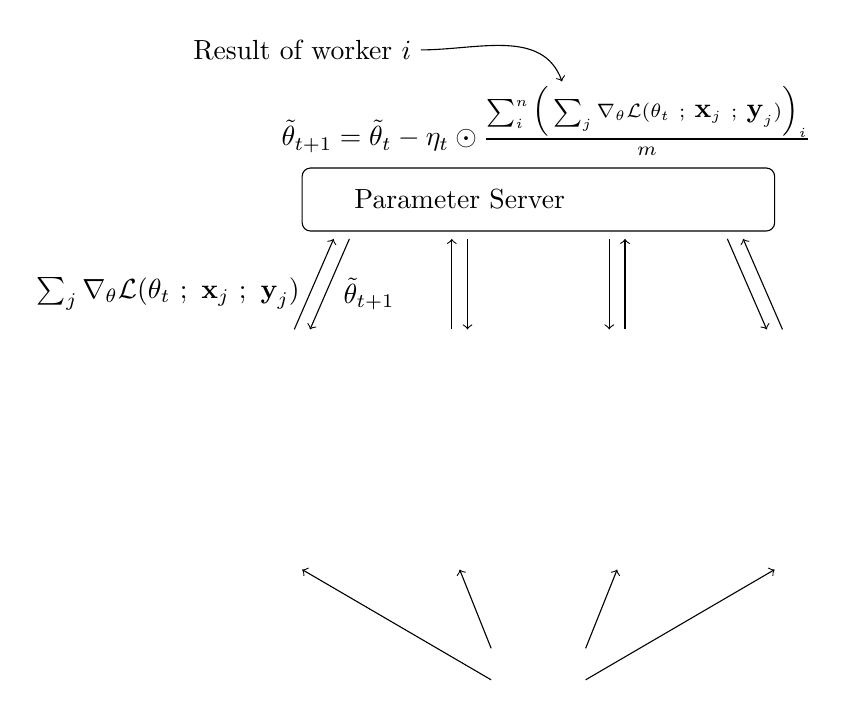
\begin{tikzpicture}
    \database at (0,-1);
    \draw[->] (-0.6,-1.5) -- (-3, -0.1);
    \draw[->] (-0.6,-1.1) -- (-1, -0.1);
    \draw[->] (0.6,-1.1) -- (1, -0.1);
    \draw[->] (0.6,-1.5) -- (3, -0.1);
    \datashard at (-3,0.6);
    \datashard at (-1,0.6);
    \datashard at (1,0.6);
    \datashard at (3,0.6);
    \minibatch at (-3, 1.7);
    \minibatch at (-1, 1.7);
    \minibatch at (1, 1.7);
    \minibatch at (3, 1.7);
    \neuralnet at (3,2.35);
    \neuralnet at (1,2.35);
    \neuralnet at (-1,2.35);
    \neuralnet at (-3,2.35);
    % Draw the parameter server.
    \draw[rounded corners=3pt] (-3, 5) rectangle ++(6,-0.8);
    \node (pslabel) at (-1, 4.6) {Parameter Server};
    \node (psequation) at (0.1, 5.6) {$\tilde{\theta}_{t+1} = \tilde{\theta}_t - \eta_t \odot \frac{\sum_i^n \Big( \sum_j \nabla_\theta \mathcal{L}(\theta_t~;~\textbf{x}_j~;~\textbf{y}_j) \Big)_i}{m}$};
    \node (description) at (-3, 6.5) {Result of worker $i$};
    \draw (description) edge[out=0, in=110, ->] (0.3, 6.1);
    % Draw the lines.
    \neuralnetclean at (1.8, 4.6);
    \draw[->] (-3.1, 2.95) -- (-2.6, 4.1);
    \draw[<-] (-2.9, 2.95) -- (-2.4, 4.1);
    \draw[->] (-1.1, 2.95) -- (-1.1, 4.1);
    \draw[<-] (-0.9, 2.95) -- (-0.9, 4.1);
    \draw[->] (1.1, 2.95) -- (1.1, 4.1);
    \draw[<-] (0.9, 2.95) -- (0.9, 4.1);
    \draw[->] (3.1, 2.95) -- (2.6, 4.1);
    \draw[<-] (2.9, 2.95) -- (2.4, 4.1);
    % Draw the labels.
    \node (commit) at (-2.15, 3.4) {$\tilde{\theta}_{t+1}$};
    \node (pull) at (-4.7, 3.4) {$\sum_j \nabla_\theta \mathcal{L}(\theta_t~;~\textbf{x}_j~;~\textbf{y}_j)$};
    % More labels.
  \end{tikzpicture}
  \caption{Distributed mini-batch data parallelism with $n$ parallel workers, with a total mini-batch size of $m$. At the start, the data is split into $n$ partitions, and all workers get a copy of the central model with parameterization $\tilde{\theta}_0$. When the training starts, every worker $i$ computes the accumulated gradient $\sum_j \nabla_\theta \mathcal{L}(\theta_t~;~\textbf{x}_j~;~\textbf{y}_j)$ based on its part of the mini-batch, which is then \emph{commited} (send) to the parameter server. After the parameter server receives all accumulated gradients, it averages them, and then applies the batched gradient to the model in order to produce $\tilde{\theta}_{t+1}$. After the new parametrization is available, the workers will be able to \emph{pull} (download) $\tilde{\theta}_{t+1}$, and repeat the procedure described above.}
  \label{fig:distributed_mini_batch_parallelism}
\end{figure}

This of course begs the question, \emph{can we eliminate the need for a locking mechanism to prevent unnecessary waits of the workers}? There are some significant initial counter-arguments against removing the synchronization barrier. The most profound issue by removing the synchronization barrier, and thus obtaining \emph{Asynchronous Data Parallelism}, is that the parameter server will incorperate gradients using a simple queuing model (FIFO) based on older parameterizations of the central variable, as shown in Figure~\ref{fig:intro_asyn_data_parallelism}.

\begin{figure}[H]
  \centering
  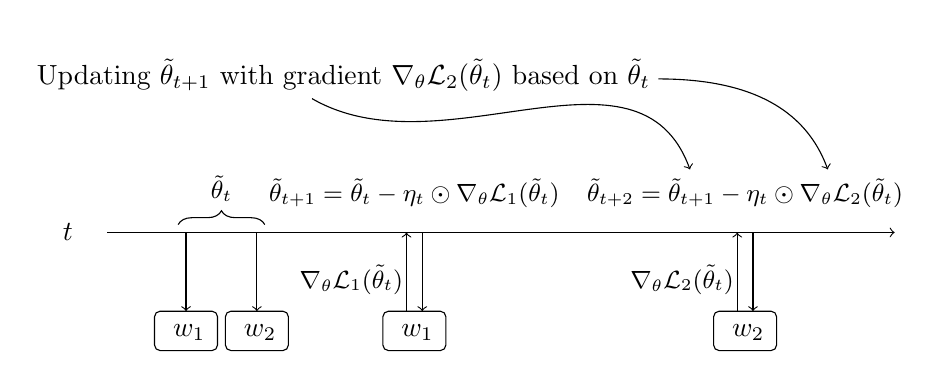
\begin{tikzpicture}
    % Draw the timeline.
    \node at (-5.5, 0) {$t$};
    \draw[->] (-5, 0) -- (5, 0);

    % Draw the first pull of the workers.
    \draw[->] (-4, 0) -- (-4, -1);
    \draw[->] (-3.1, 0) -- (-3.1, -1);
    \draw[rounded corners=2pt] (-4.4, -1) rectangle (-3.6, -1.5) node[pos=.55] {$w_1$};
    \draw[rounded corners=2pt] (-3.5, -1) rectangle (-2.7, -1.5) node[pos=.55] {$w_2$};
    % Draw initial pull decoration.
    \draw [decorate,decoration={brace,amplitude=5pt}]
    (-4.1, 0.1) -- (-3, 0.1) node [black,midway,yshift=13pt] {\small $\tilde{\theta}_t$};

    % Draw first commit and pull.
    \draw[->] (-1, 0) --(-1, -1);
    \draw[<-] (-1.2, 0) -- (-1.2, -1);
    \node at (-1.9, -0.6) {\small $\nabla_\theta \mathcal{L}_1(\tilde{\theta}_t)$};
    \draw[rounded corners=2pt] (-1.1 - 0.4, -1) rectangle (-1.1 + 0.4, -1.5) node[pos=.55] {$w_1$};
    \node at (-1.1, 0.5) {\small $\tilde{\theta}_{t+1} = \tilde{\theta}_t - \eta_t \odot \nabla_\theta \mathcal{L}_1(\tilde{\theta}_t)$};

    % Draw second commit and pull.
    \draw[<-] (3, 0) --(3, -1);
    \draw[->] (3.2, 0) -- (3.2, -1);
    \node at (2.3, -0.6) {\small $\nabla_\theta \mathcal{L}_2(\tilde{\theta}_t)$};
    \draw[rounded corners=2pt] (3.1 - 0.4, -1) rectangle (3.1 + 0.4, -1.5) node[pos=.55] {$w_2$};
    \node at (3.1, 0.5) {\small $\tilde{\theta}_{t+2} = \tilde{\theta}_{t+1} - \eta_t \odot \nabla_\theta \mathcal{L}_2(\tilde{\theta}_t)$};

    % Write description.
    \node at (-2, 2) {Updating $\tilde{\theta}_{t+1}$ with gradient $\nabla_\theta \mathcal{L}_2(\tilde{\theta}_t)$ based on $\tilde{\theta}_t$};
    \draw (-2.4, 1.7) edge[out=-30, in=110, ->] (2.4, 0.8);
    \draw (2, 1.95) edge[out=0, in=110, ->] (4.15, 0.8);
  \end{tikzpicture}
  \caption{In Asynchronous Data Parallelism workers compute and commit gradients to the parameter server asynchronously. This has as a side-effect that some workers are computing, and thus committing, gradients based on old values. These gradients are called \emph{stale gradients} in literature. In this particular example there are 2 workers $w_1$, and $w_2$. At the start optimization process, the pull the most recent parameterization from the parameter server $\tilde{\theta}_t$. Now all workers start computing the gradients asynchronously based on the pulled parametrization. However, since the parameter server incorperates gradients into the center variable asynchronously as a simple queuing (FIFO) model, other workers will update the center variable with gradients based on an older value, as shown in the figure above. Finally, assuming that the computing cluster is homogeneous, we can derive from this figure that the expected staleness of a gradient update is $\mathbf{E}[\tau] = (n - 1)$.}
  \label{fig:intro_asyn_data_parallelism}
\end{figure}

However, experiments have shown that removing the synchronization barrier actually allows models to converge~\cite{dean2012large, zhang2015deep, hadjis2016omnivore}, even when most workers update the central variable using a gradient based on an outdated parameterization of the central variable. An other issue, which only has been formalized recently, is \emph{Implicit Momentum} or \emph{Asynchrony Induced Momentum}~\cite{implicitmomentum}. The main reasoning behind implicit momentum, which will be discussed in detail in Section~\ref{sec:implicit_momentum}, is based on a very simple but powerful idea. The idea states that \emph{memory arizes from asynchrony}. Intuitively, this implies that ``memory'' of previous gradients is preserved due to \emph{stale gradient} updates. This can be observed directly from Figure~\ref{fig:intro_asyn_data_parallelism}, where the update of $w_2$ is actually updating the central variable with a gradient identical to $\nabla_\theta \mathcal{L}_1(\tilde{\theta}_t)$ if we assume that both workers computed the gradient based on the same input data. This is a clear indication that asynchronous data parallelism is \emph{implicitly} (because of the asynchronous nature of the approach) adding \emph{momentum} which is proportional to the number of workers, since adding more workers actually \emph{adds} more ``memory'' about previous parameterizations. The authors formalize this by probabilistically estimating the expected change between $\tilde{\theta}_{t+1}$ and $\tilde{\theta}_t$. Using some additional additional assumptions, such as the expected staleness $\mathbf{E}[\tau] = (n - 1)$, and geometrically distributed staleness, the authors are able to formalize the expected update in an asynchronous setting between update $t$ and $t + 1$, which is shown in Equation~\ref{eq:implicit_momentum}.

\begin{equation}
  \label{eq:implicit_momentum}
  \mathbf{E}[\tilde{\theta}_{t+1} - \tilde{\theta}_t] = \Bigg( 1 - \frac{1}{n} \Bigg) \mathbf{E}[\tilde{\theta}_t - \tilde{\theta}_{t-1}] - \frac{\eta}{n} \mathbf{E} \nabla_\theta \mathcal{L}(\tilde{\theta}_t~;~\textbf{x}~;~\textbf{y})
\end{equation}

Using Equation~\ref{eq:implicit_momentum}, we can immediatly derrive the term which describes the implicit momentum induced by asynchrony, which is $\big(1 - \frac{1}{n}\big)$. This result actually suggests that there is a limit to asynchronous optimization: since every problem has some optimal momentum term, which implies that there is an optimal number of asynchronous workers for a specific problem. In order to push the limits of asynchronous optimization, the authors propose various techniques to reduce the abundant amount of implicit momentum. One approach is to apply a \emph{grid-search} to find the optimal hyperparameterization for a given epoch, this also includes the number of workers. Despite that this technique finds the optimal hyperparameterization for a given epoch, the disadvantage is that after every fixed number of iterations, a grid-search of the hyperparameters has to be performed to ensure (optimal) convergence. This is actually in accordance with training in non-data parallel settings, where one starts with a smaller momentum hyperparameter because the gradients at the start will be relatively large compared to the gradients near an optimum, where usually one benifits from a larger momentum hyperparameter. From this intuition we can actually deduce that when the gradient updates are large compared to the gradients close to an optimum, an optimizer does not benifit from high parallelism because the workers are committing gradients which were based on a parametrization which is ``far'' from the current central variable, thus obtaining implicit momentum. Furthermore, one could eliminate the need for the gridsearch by constructing a distributed optimization scheme which is based on the idea described in Hypothesis~\ref{hyp:local_optimization}.

\begin{hyp}[H\ref{hyp:local_optimization}] \label{hyp:local_optimization}
  Workers only contribute efficiently to the central objective when they commit gradients which are based on variables close to the central variable.
\end{hyp}

This implies that in the precense of high parallelism, only gradient updates which are based on variables close to the \emph{current} central variable matter. This intuition is strengthened in Figure~\ref{fig:async_momentum}, where a straggler is causing the central variable to converge to a different solution as opposed to the one it was heading to first. A lot of methodologies have been suggested to handle the stragler problem, however, most approaches suggest a synchronous bounded staleness approach~\cite{cipar2013solving, ho2013more}. As a result, the error introduced by staleness is limited~\cite{ho2013more}. Nevertheless, in gradient-based approaches, the straggler problem can be approached from a different perspective. By incorperating Hypothesis~\ref{hyp:local_optimization}, we could eliminate additional engineering efforts since stale updates, and thus straglers, are built in the optimization procedure.

\begin{figure}[H]
  \centering
  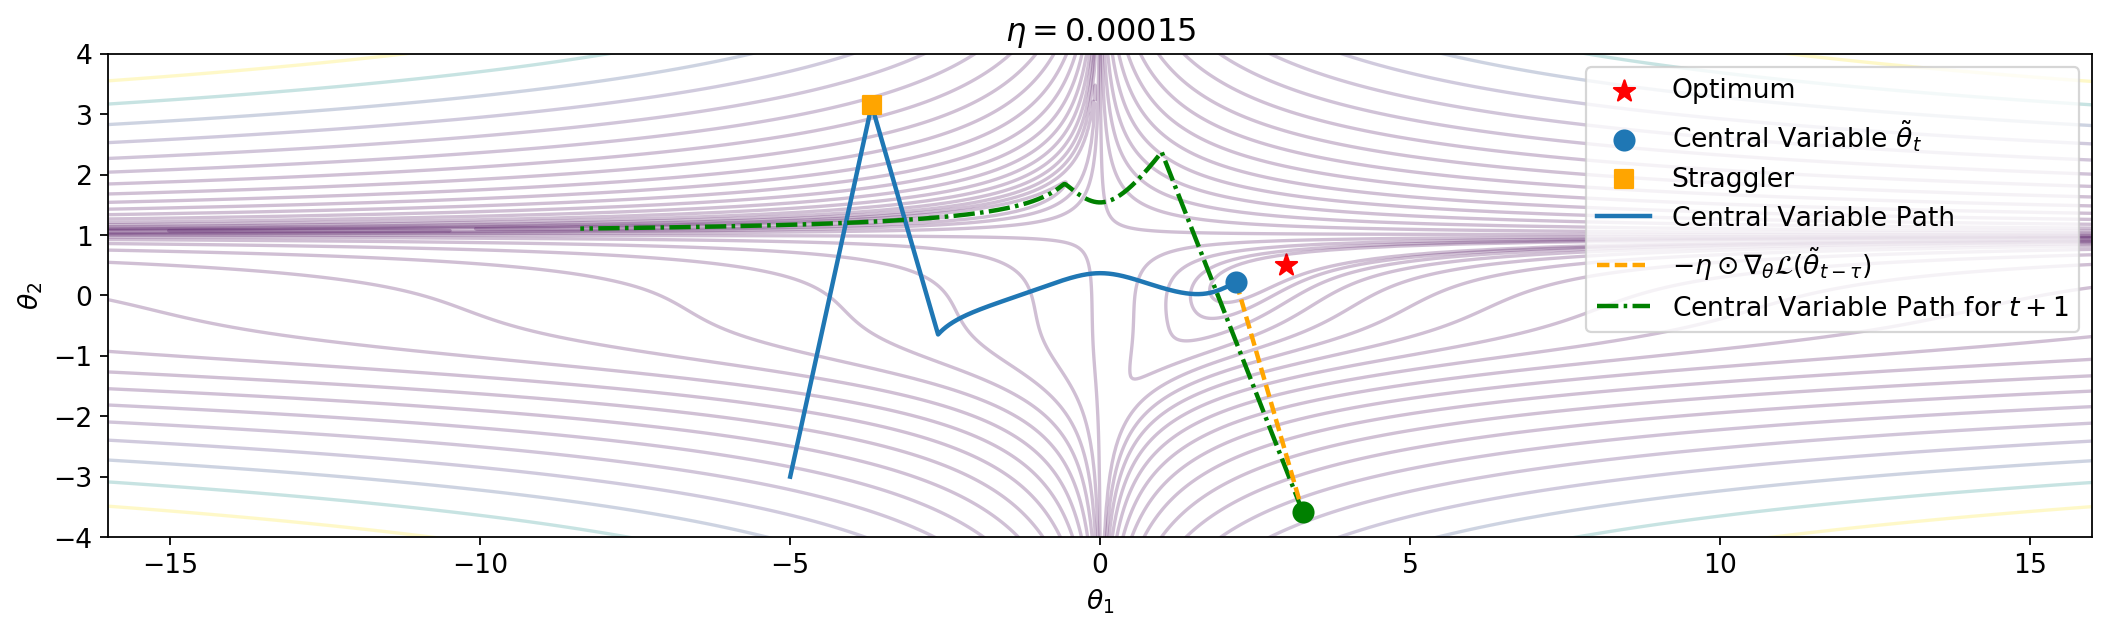
\includegraphics[width=\textwidth]{resources/images/async_straggler}
  \caption{Asynchronous optimization procedure applied to Beale's function. In this experiment we introduce a straggler programatically (square) at the start of the optimization process. Despite the fact that this is a low probability event (large staleness compared to the number of workers) in real-world situtations, the effect we describe here is present in any form of asynchronous optimization. When the straggler in this figure \emph{commits} its gradient update to the parameter server, the central variable $\tilde{\theta}_t$ will be updated using $-\eta_t \odot \nabla_\theta \mathcal{L}(\tilde{\theta}_{t - \tau})$ with staleness $\tau$ to form $\tilde{\theta}_{t+1}$. This update causes the central variable to converge to a different optimum, and additionially, increases the error of the central variable (green circle). Furthermore, to actually converge to the other optimum, additional computational work has to be performed. This situation drives our intuition presented in Hypothesis~\ref{hyp:local_optimization}.}
  \label{fig:async_momentum}
\end{figure}

One could of course argue, why not use a smaller number of workers since we are annealing the gradients which are based on non-local variables anyway, thus wasting computational resources on those machines? This is certainly a valid argument. However, let us first consider the hyperparameter grid-search approach suggested by~\cite{implicitmomentum}. As mentioned above, despite the fact that the grid-search technique will find the optimal hyperparameters for the current parameterization, it doesn't mean that these hyperparameters are still optimal during the duration of the training process. Furthermore, to actually obtain the optimal hyperparameters, some certain amount of time needs to be spent in order to find them. This is actually quite problematic, since one actually wishes to reduce training time by applying data parallel techniques. In our approach, which will be discussed extensively in Chapter~\ref{chapter:asynchronous_distributed_adaptive_gradients}, this is not the case since the gradients will be annealed dynamically based on the curvature of the error space and current parametrization of the central variable, i.e., there is no need for a hyperparameter grid-search during the training process.

\newpage

Now some general approaches and important issues regarding data parallelism have been addressed, and the reader has gained some intuition on the subject, we can formalize data parallelism and use the notation in the following chapters. In order to formalize data parallelism, let us assume we have a dataset $D$, which contains our training data, and that we are able to distribute dataset $D$ over $n$ different workers $\mathcal{W} = \{w_1, \ldots, w_n\}$. Where every worker $w_i \in \mathcal{W}$ holds a copy of the central model, thus, a copy of the parameterization of the central model $\tilde{\theta}_0$. Furthermore, we denote the parametrization of a particular worker $k$ at time $t$ by $\theta_t^k$. Of course, if a worker wants to contribute to the optimization of the central model, the worker needs to be able to relay update information and retrieve the most recent parameterization of the central model. This is done by instantiating a parameter server, where workers will be able to \emph{commit} their updates, and \emph{pull} the most recent parameterization of the central model. The parameterization of the central model is called the \emph{central variable}, which we denote by $\tilde{\theta}_t$. In the final preperation step, before the actual training starts, $\mathcal{D}$ will be split into roughly $n$ equally sized partitions $\mathcal{P} = \{p_1, \ldots, p_n\}$, where $\left\vert{p_i}\right\vert \approx \frac{1}{\left\vert{\mathcal{D}}\right\vert}$, and where $p_i$ will be assigned to the corresponding worker $w_i$.\\

In general, all data parallel approaches share a similar training procedure, i.e., every worker computes some variable which is communicated with the parameter server to update the central model. In most cases, this variable represents some change $\Delta\theta$ which needs to be applied to the central variable $\tilde{\theta}_t$. However, some approaches such as~\cite{zhang2015deep}, actually require that the complete worker parametrization $\theta^k_t$ is sent to the parameter server. To abstract this specific optimizer detail, we denote the variable that is sent to the parameter server by $v$. This procedure is described in Algorithm~\ref{algo:data_parallelism_worker} and~\ref{algo:data_parallelism_parameter_server}.

\begin{figure}[H]
  \centering
  % Define database shape.
  \def\database at (#1,#2){
    \draw (#1,#2) ellipse (0.5 and 0.15);
    \draw (#1 - 0.5, #2) -- (#1 - 0.5, #2 - 1);
    \draw (#1 + 0.5, #2) -- (#1 + 0.5, #2 - 1);
    \draw (#1 - 0.5, #2 - 1/3) arc (180:360:0.5 and 0.15);
    \draw (#1 - 0.5, #2 - 2/3) arc (180:360:0.5 and 0.15);
    \draw (#1 - 0.5, #2 - 1) arc (180:360:0.5 and 0.15);
  }
  % Define datashard shape.
  \def\datashard at (#1,#2){
    \draw (#1,#2) ellipse (0.5 and 0.15);
    \draw (#1 - 0.5, #2) -- (#1 - 0.5, #2 - 1/3);
    \draw (#1 + 0.5, #2) -- (#1 + 0.5, #2 - 1/3);
    \draw (#1 - 0.5, #2 - 1/3) arc (180:360:0.5 and 0.15);
  }
  % Define the neural network shape.
  \def\neuralnet at (#1,#2){
    % Draw node bounding box.
    \draw[rounded corners=3pt] (#1 - 0.7,#2 + 0.5) rectangle ++(1.4,-0.95);
    % Draw fully connected lines.
    \draw[gray] (#1 + 0.25,#2) -- (#1 - 0.375, #2 + 0.25);
    \draw[gray] (#1 + 0.25,#2) -- (#1 - 0.125, #2 + 0.25);
    \draw[gray] (#1 + 0.25,#2) -- (#1 + 0.125, #2 + 0.25);
    \draw[gray] (#1 + 0.25,#2) -- (#1 + 0.375, #2 + 0.25);
    \draw[gray] (#1 + 0.5,#2) -- (#1 - 0.375, #2 + 0.25);
    \draw[gray] (#1 + 0.5,#2) -- (#1 - 0.125, #2 + 0.25);
    \draw[gray] (#1 + 0.5,#2) -- (#1 + 0.125, #2 + 0.25);
    \draw[gray] (#1 + 0.5,#2) -- (#1 + 0.375, #2 + 0.25);
    \draw[gray] (#1,#2) -- (#1 - 0.375, #2 + 0.25);
    \draw[gray] (#1,#2) -- (#1 - 0.125, #2 + 0.25);
    \draw[gray] (#1,#2) -- (#1 + 0.125, #2 + 0.25);
    \draw[gray] (#1,#2) -- (#1 + 0.375, #2 + 0.25);
    \draw[gray] (#1 - 0.25,#2) -- (#1 - 0.375, #2 + 0.25);
    \draw[gray] (#1 - 0.25,#2) -- (#1 - 0.125, #2 + 0.25);
    \draw[gray] (#1 - 0.25,#2) -- (#1 + 0.125, #2 + 0.25);
    \draw[gray] (#1 - 0.25,#2) -- (#1 + 0.375, #2 + 0.25);
    \draw[gray] (#1 - 0.5,#2) -- (#1 - 0.375, #2 + 0.25);
    \draw[gray] (#1 - 0.5,#2) -- (#1 - 0.125, #2 + 0.25);
    \draw[gray] (#1 - 0.5,#2) -- (#1 + 0.125, #2 + 0.25);
    \draw[gray] (#1 - 0.5,#2) -- (#1 + 0.375, #2 + 0.25);
    \draw[gray] (#1 + 0.25,#2) -- (#1 + 0.125, #2 - 0.25);
    \draw[gray] (#1 + 0.25,#2) -- (#1 - 0.125, #2 - 0.25);
    \draw[gray] (#1 + 0.5,#2) -- (#1 + 0.125, #2 - 0.25);
    \draw[gray] (#1 + 0.5,#2) -- (#1 - 0.125, #2 - 0.25);
    \draw[gray] (#1,#2) -- (#1 + 0.125, #2 - 0.25);
    \draw[gray] (#1,#2) -- (#1 - 0.125, #2 - 0.25);
    \draw[gray] (#1 - 0.25,#2) -- (#1 + 0.125, #2 - 0.25);
    \draw[gray] (#1 - 0.25,#2) -- (#1 - 0.125, #2 - 0.25);
    \draw[gray] (#1 - 0.5,#2) -- (#1 + 0.125, #2 - 0.25);
    \draw[gray] (#1 - 0.5,#2) -- (#1 - 0.125, #2 - 0.25);
    % Define input layer.
    \draw[fill=white] (#1 - 0.375,#2 + 0.25) circle (1pt);
    \draw[fill=white] (#1 - 0.125,#2 + 0.25) circle (1pt);
    \draw[fill=white] (#1 + 0.125,#2 + 0.25) circle (1pt);
    \draw[fill=white] (#1 + 0.375,#2 + 0.25) circle (1pt);
    % Define hidden layer.
    \draw[fill=white] (#1 - 0.5,#2) circle (1pt);
    \draw[fill=white] (#1 - 0.25,#2) circle (1pt);
    \draw[fill=white] (#1,#2) circle (1pt);
    \draw[fill=white] (#1 + 0.25,#2) circle (1pt);
    \draw[fill=white] (#1 + 0.5,#2) circle (1pt);
    % Define output layer.
    \draw[fill=white] (#1 - 0.125,#2 - 0.25) circle (1pt);
    \draw[fill=white] (#1 + 0.125,#2 - 0.25) circle (1pt);
  }
  \def\neuralnetclean at (#1,#2){
    \draw[gray] (#1 + 0.25,#2) -- (#1 - 0.375, #2 + 0.25);
    \draw[gray] (#1 + 0.25,#2) -- (#1 - 0.125, #2 + 0.25);
    \draw[gray] (#1 + 0.25,#2) -- (#1 + 0.125, #2 + 0.25);
    \draw[gray] (#1 + 0.25,#2) -- (#1 + 0.375, #2 + 0.25);
    \draw[gray] (#1 + 0.5,#2) -- (#1 - 0.375, #2 + 0.25);
    \draw[gray] (#1 + 0.5,#2) -- (#1 - 0.125, #2 + 0.25);
    \draw[gray] (#1 + 0.5,#2) -- (#1 + 0.125, #2 + 0.25);
    \draw[gray] (#1 + 0.5,#2) -- (#1 + 0.375, #2 + 0.25);
    \draw[gray] (#1,#2) -- (#1 - 0.375, #2 + 0.25);
    \draw[gray] (#1,#2) -- (#1 - 0.125, #2 + 0.25);
    \draw[gray] (#1,#2) -- (#1 + 0.125, #2 + 0.25);
    \draw[gray] (#1,#2) -- (#1 + 0.375, #2 + 0.25);
    \draw[gray] (#1 - 0.25,#2) -- (#1 - 0.375, #2 + 0.25);
    \draw[gray] (#1 - 0.25,#2) -- (#1 - 0.125, #2 + 0.25);
    \draw[gray] (#1 - 0.25,#2) -- (#1 + 0.125, #2 + 0.25);
    \draw[gray] (#1 - 0.25,#2) -- (#1 + 0.375, #2 + 0.25);
    \draw[gray] (#1 - 0.5,#2) -- (#1 - 0.375, #2 + 0.25);
    \draw[gray] (#1 - 0.5,#2) -- (#1 - 0.125, #2 + 0.25);
    \draw[gray] (#1 - 0.5,#2) -- (#1 + 0.125, #2 + 0.25);
    \draw[gray] (#1 - 0.5,#2) -- (#1 + 0.375, #2 + 0.25);
    \draw[gray] (#1 + 0.25,#2) -- (#1 + 0.125, #2 - 0.25);
    \draw[gray] (#1 + 0.25,#2) -- (#1 - 0.125, #2 - 0.25);
    \draw[gray] (#1 + 0.5,#2) -- (#1 + 0.125, #2 - 0.25);
    \draw[gray] (#1 + 0.5,#2) -- (#1 - 0.125, #2 - 0.25);
    \draw[gray] (#1,#2) -- (#1 + 0.125, #2 - 0.25);
    \draw[gray] (#1,#2) -- (#1 - 0.125, #2 - 0.25);
    \draw[gray] (#1 - 0.25,#2) -- (#1 + 0.125, #2 - 0.25);
    \draw[gray] (#1 - 0.25,#2) -- (#1 - 0.125, #2 - 0.25);
    \draw[gray] (#1 - 0.5,#2) -- (#1 + 0.125, #2 - 0.25);
v    \draw[gray] (#1 - 0.5,#2) -- (#1 - 0.125, #2 - 0.25);
    % Define input layer.
    \draw[fill=white] (#1 - 0.375,#2 + 0.25) circle (1pt);
    \draw[fill=white] (#1 - 0.125,#2 + 0.25) circle (1pt);
    \draw[fill=white] (#1 + 0.125,#2 + 0.25) circle (1pt);
    \draw[fill=white] (#1 + 0.375,#2 + 0.25) circle (1pt);
    % Define hidden layer.
    \draw[fill=white] (#1 - 0.5,#2) circle (1pt);
    \draw[fill=white] (#1 - 0.25,#2) circle (1pt);
    \draw[fill=white] (#1,#2) circle (1pt);
    \draw[fill=white] (#1 + 0.25,#2) circle (1pt);
    \draw[fill=white] (#1 + 0.5,#2) circle (1pt);
    % Define output layer.
    \draw[fill=white] (#1 - 0.125,#2 - 0.25) circle (1pt);
    \draw[fill=white] (#1 + 0.125,#2 - 0.25) circle (1pt);
  }
  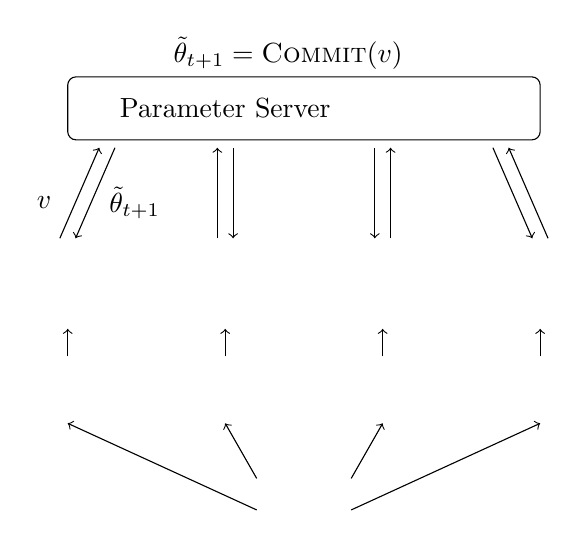
\begin{tikzpicture}
    \database at (0,0);
    \draw[->] (-0.6,-0.5) -- (-3, 0.6);
    \draw[->] (-0.6,-0.1) -- (-1, 0.6);
    \draw[->] (0.6,-0.1) -- (1, 0.6);
    \draw[->] (0.6,-0.5) -- (3, 0.6);
    \datashard at (-3,1.2)
    \datashard at (-1,1.2);
    \datashard at (1,1.2);
    \datashard at (3,1.2);
    \draw[->] (-3, 1.45) -- (-3, 1.8);
    \draw[->] (-1, 1.45) -- (-1, 1.8);
    \draw[->] (1, 1.45) -- (1, 1.8);
    \draw[->] (3, 1.45) -- (3, 1.8);
    \neuralnet at (3,2.35);
    \neuralnet at (1,2.35);
    \neuralnet at (-1,2.35);
    \neuralnet at (-3,2.35);
    % Draw the parameter server.
    \draw[rounded corners=3pt] (-3, 5) rectangle ++(6,-0.8);
    \node (pslabel) at (-1, 4.6) {Parameter Server};
    \node (psequation) at (-0.2, 5.3) {$\tilde{\theta}_{t+1} = \textsc{Commit}(v)$};
    % Draw the lines.
    \neuralnetclean at (1.8, 4.6);
    \draw[->] (-3.1, 2.95) -- (-2.6, 4.1);
    \draw[<-] (-2.9, 2.95) -- (-2.4, 4.1);
    \draw[->] (-1.1, 2.95) -- (-1.1, 4.1);
    \draw[<-] (-0.9, 2.95) -- (-0.9, 4.1);
    \draw[->] (1.1, 2.95) -- (1.1, 4.1);
    \draw[<-] (0.9, 2.95) -- (0.9, 4.1);
    \draw[->] (3.1, 2.95) -- (2.6, 4.1);
    \draw[<-] (2.9, 2.95) -- (2.4, 4.1);
    % Draw the labels.
    \node (commit) at (-2.15, 3.4) {$\tilde{\theta}_{t+1}$};
    \node (pull) at (-3.3, 3.4) {$v$};
    % More labels.
  \end{tikzpicture}
  \caption{Schematic representation of a data parallel approach. In this methodology we spawn $n$ workers (not necessarily on different machines), and assign a data shard (partition) of the dataset to every worker. Using this data shard, a worker $i$ will iterate through all mini-batches to produce a gradient, $\nabla_\theta \mathcal{L}_i(x)$, for every mini-batch $\textbf{m}$. Next, a variable $v$ is constructed on the worker which is send to the parameter server. The parameter server will incorperate the variable using a~\textsc{Commit} mechanism to produce the next central parametrization $\tilde{\theta}_{t+1}$.}
  \label{fig:introduction_data_parallelism_schematic}
\end{figure}

Nevertheless, the most common and one of the earliest asynchronous optimization algorithm is \textsc{downpour}~\cite{dean2012large}. In this Master Thesis, we use \textsc{downpour} as a baseline performance indicator for all our experiments with other distributed optimization algorithms. In essence, workers are continuously committing gradients to the parameter server using Equation~\ref{eq:downpour_worker}. After a gradient has been committed to the parameter server, the worker will \emph{pull} the most recent parameterization from the parameter server in order to be consistent with the updates of other workers, as in Algorithm~\ref{algo:data_parallelism_worker} and~\ref{algo:data_parallelism_parameter_server}.

\begin{equation}
  \label{eq:downpour_worker}
  \Delta \theta^k = - \eta_t \odot \nabla_\theta \mathcal{L}(\tilde{\theta}_{t-\tau}~;~\textbf{x}~;~\textbf{y})
\end{equation}

\newpage

Once the parameter server received the update $\Delta\theta^k$ from worker $k$, the parameter server will simply add (since the worker already negated the gradient) the update to the current central variable in order to produce $\tilde{\theta}_{t+1}$, this is described by Equation~\ref{eq:downpour_parameter_server}.

\begin{equation}
  \label{eq:downpour_parameter_server}
  \tilde{\theta}_{t+1} = \tilde{\theta}_t + \Delta \theta^k
\end{equation}

Furthermore, in order to examine the scaling abilities of the optimization algorithms we discuss in the following chapters, we need a measure to express how well they are performing in a given scenario. To measure this, one could use more traditional metrics such as \emph{statistical efficiency} and \emph{hardware efficiency}~\cite{hadjis2016omnivore, implicitmomentum}.\\

\textbf{Statistical efficiency} (SE) describes the number of iterations that are required to obtain a desired result. In the context of Machine Learning, statistical efficiency describes the number of model updates that have to be performed in order to acquire a desired accuracy. However, in order to obtain some metric about a specific optimization algorithm, we need a baseline to compare against. As stated above, the baseline algorithm we use in this work is \textsc{downpour}. Once we evaluated an algorithm $\epsilon$, we compute the statistical efficiency of $\epsilon$ compared to \textsc{downpour}, as described by Equation~\ref{eq:statistical_efficiency}.

\begin{equation}
  \label{eq:statistical_efficiency}
  \frac{SE(\textsc{downpour})}{SE(\epsilon)}
\end{equation}

\textbf{Hardware efficiency} (HE) on the other hand, describes the amount of time it takes to execute a single iteration of a loop. In our work, this denotes the time it takes to complete a \emph{single} epoch. Nonetheless, during this work, we experimented with several optimization algorithms which actually compute several gradients locally, and preprocess them before transmitting the update to the parameter server~\cite{zhang2015deep}. In these cases, if someone would employ statistical or hardware efficiency to obtain a performance indicator compared to an other algorithm, they will have a clear advantage since a significantly smaller number of central variable updates occur. Furthermore, usually these algorithms also spend less time consuming all the data since parameter server updates occur less frequent. Moreover, the network is also less saturated due to the reduced number of parameter server updates. In order to have a non-biased metric among different distributed optimization algorithms, we should look at the time it takes to obtain a desired accuracy. We call this \emph{temporal efficiency}.\\

\textbf{Temporal efficiency} (TE) characterizes the amount of time a process, or a collection of processes, requires in order to obtain a desired accuracy. Temporal efficiency is in effect propertional to statistical efficiency, i.e., $SE(\epsilon) \propto TE(\epsilon)$. However, this is only the case when algorithm $\epsilon$ actually transmits an update to the parameter server after a worker computed a gradient (in an asynchronous setting). This is in contrast with algorithms such as~\cite{zhang2015deep}, where some additional samples are evaluated locally, before an update is transmitted to the parameter server.

\newpage
\vspace*{\fill}

% Define the general data parallel worker algorithm.
\begin{algorithm}
  \caption{Describes the general asynchronous optimization procedure of a worker in a data parallel setting. The worker will be identified with a certain index $k$, the other parameter $p_k \in \mathcal{P}$, is the data partition which has been assigned to worker $k$.}
  \label{algo:data_parallelism_worker}
  \begin{algorithmic}[1]
    \Procedure{Worker}{$k$, $p_k$}
    \State $\theta^k_0 \gets \Call{Pull}{ }$
    \State $t \gets 0$
    \While{$\textbf{not}$ converged}
    \State $\textbf{m} \gets \Call{FetchNextMiniBatch}{p_k}$
    \State $\theta^k_{t + 1} \gets \theta^k_t - \eta_t \odot \nabla_\theta \mathcal{L}(\theta^k_t~;~\textbf{m})$ \Comment{Optimization step, could be \cite{kingma2014adam}, or other optimizer.}
    \State $v \gets \Call{PrepareCommit}{ }$
    \State $\Call{Commit}{v}$
    \State $\theta^k_t \gets \Call{Pull}{ }$
    \State $t \gets t + 1$
    \EndWhile
    \EndProcedure
  \end{algorithmic}
\end{algorithm}

\vspace*{3cm}

% Define the general commit update mechanism.
\begin{algorithm}
  \caption{Intialization and variable handling procedures of a parameter server. Before the distributed optimization starts, the \textsc{IntializeParameterServer} procedure is called to initialize the local parameters, given the parametrization $\theta$ of the specified model. We would like to note that $t$ maintained by the parameter server, is different from the $t$ variable specified in Algorithm~\ref{algo:data_parallelism_worker}.}
  \label{algo:data_parallelism_parameter_server}
  \begin{algorithmic}[1]
    \Procedure{IntializeParameterServer}{$\theta$}
    \State $\tilde{\theta}_0 \gets \theta$
    \State $t \gets 0$
    \EndProcedure
    \State
    \Procedure{Commit}{$v$}
    \State $\tilde{\theta}_{t + 1} \gets \Call{ApplyCommit}{v}$
    \State $t \gets t + 1$
    \EndProcedure
    \State
    \Procedure{Pull}{ }
    \State \Return $\tilde{\theta}_t$
    \EndProcedure
  \end{algorithmic}
\end{algorithm}

\vspace*{\fill}

\newpage

\section{Problem Statement}
\label{sec:problem_statement}

In recent years it has been shown that being able to train large deep neural networks on vasts amount of data yield state-of-the-art classification performance. However, training these models usually takes days, or in some cases, even weeks. In order to significantly reduce the training time of these models, Jeff Dean (Google) introduced a new paradigm to train neural networks in a distributed fashion, i.e., model – and data parallelism, which is an initial attempt to tackle this problem.\\

Despite the relatively old research (2012), few efforts have been made to fully understand the implications, or to significantly improve the parallel gradient descent algorithm (\textsc{downpour}) proposed by Dean et al. Furthermore, most research focusses on limiting the error introduced by staleness by introducing some synchronization barrier, and thus limiting the amount of asynchrony. Despite this, only recently a sound theoretical argument has been made to understand asynchronous data parallelism~\cite{implicitmomentum}. Using this, and understanding this contribution, we try to push the limits of asynchronous data parallelism even further.\\

As stated above, being able to train a model on a vast amount of data generally improves the statistical performance of a model since the model will have access to many (different) examples to train on. This is in particular the case at CERN, where the experiments collected in the order of 100 PetaBytes of particle collisions in the past years. Machine Learning approaches, and Deep Learning in particular, could potentially help in data reconstruction in the upcoming runs of LHC where particles will generate a huge amount of hits in the detector where it would be infeasible to reconstruct the particle tracks using traditional techniques (combination of a Kalman filter and Runge–Kutta methods). However, due to the petabyte scale of the data, current data parallelism will not be able to train the model in a reasonable amount of time. Therefore, we think it is important to push the current limits of data parallelism even further in order to reduce the overal training time even further.

\begin{figure}[H]
\centering
\begin{subfigure}{.5\textwidth}
  \centering
  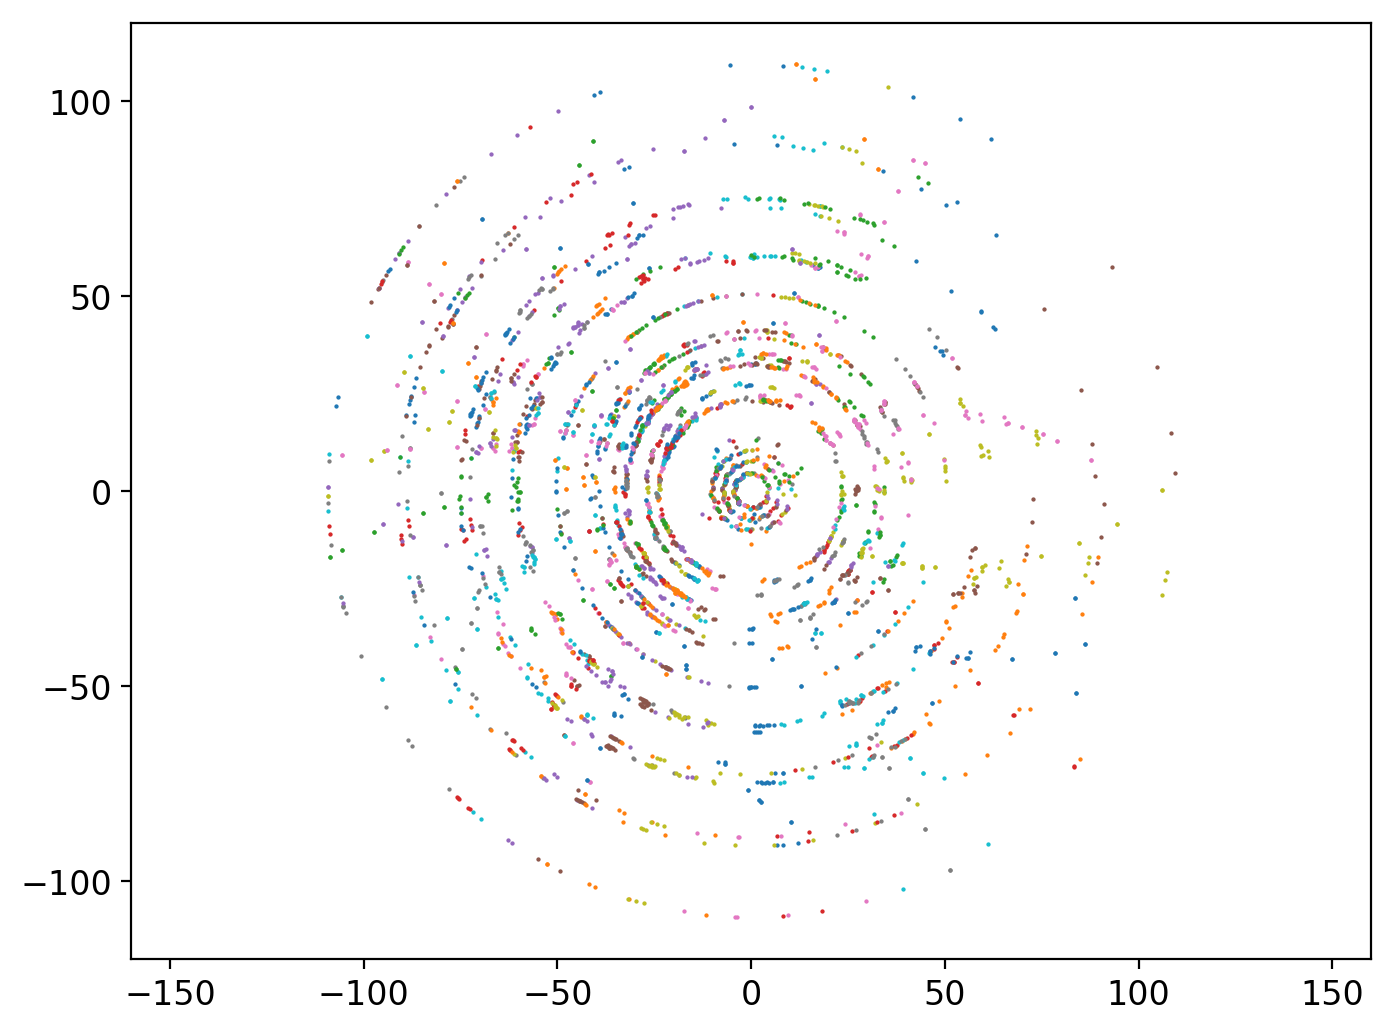
\includegraphics[width=\linewidth]{resources/images/problem_statement_cms_front}
  \caption{Front-view of the CMS detector.}
  \label{fig:problem_statement_cms_front}
\end{subfigure}%
\begin{subfigure}{.5\textwidth}
  \centering
  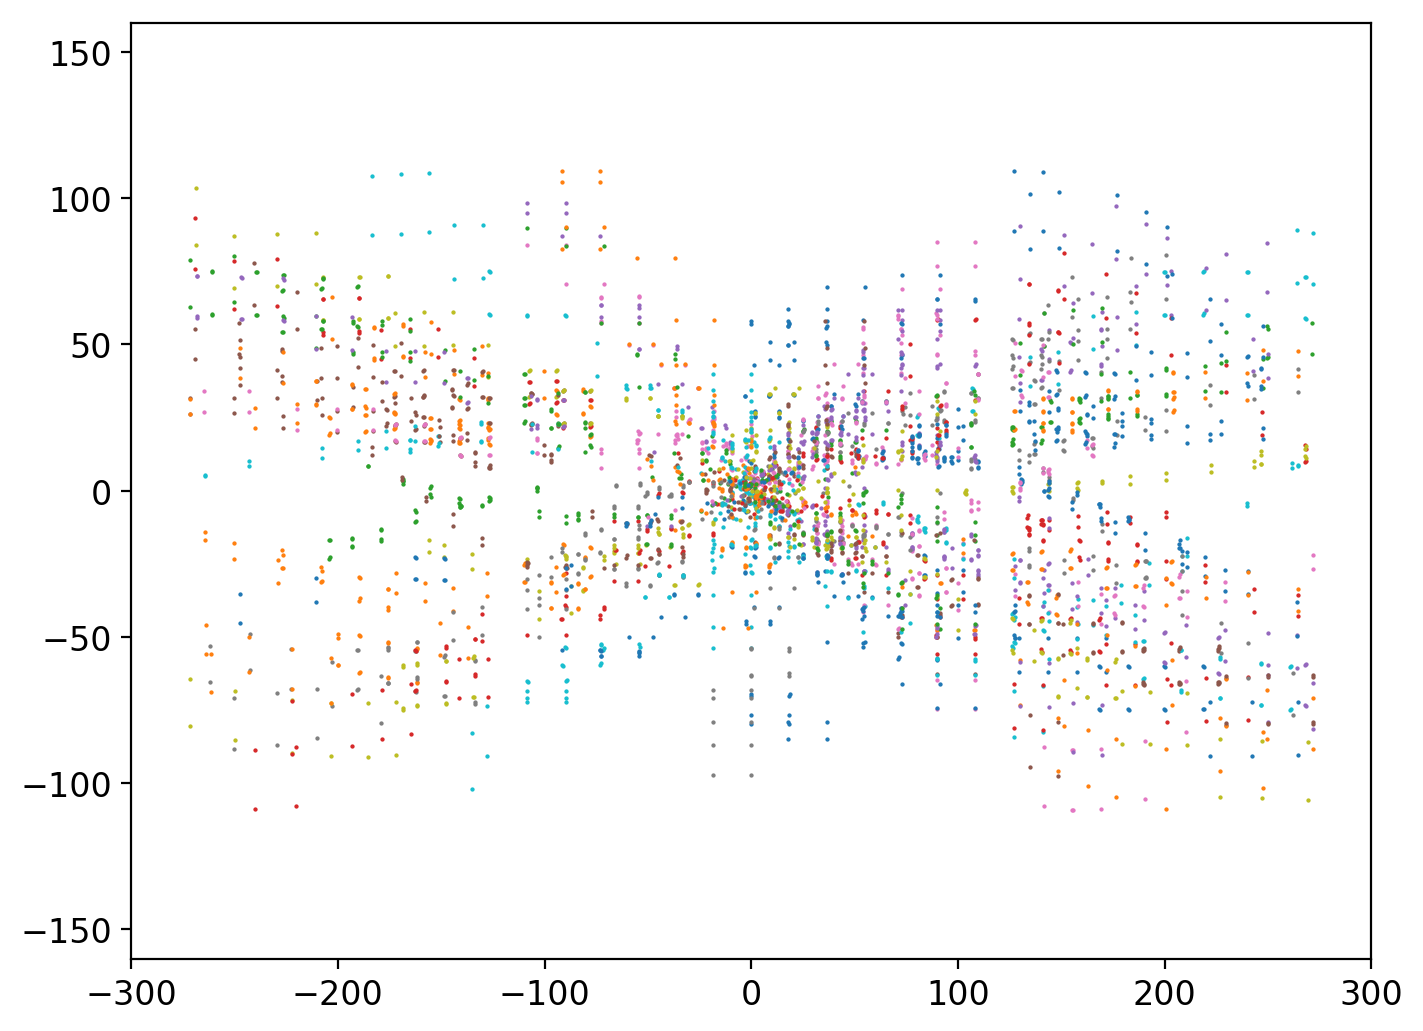
\includegraphics[width=\linewidth]{resources/images/problem_statement_cms_side}
  \caption{Side-view of the CMS detector.}
  \label{fig:problem_statement_cms_side}
\end{subfigure}
\caption{Reconstructed particle hits in the CMS detector. The collision point (vertex) is originated at (0,0,0). The inner part of the detector is called the \emph{pixel silicon} detector. This is a high resolution tracking mechanism which is able to handle the highly saturated environment of the inner part of the detector. The more outward part in this particular figure is the \emph{silicon strip} detector. The silicon strip detector basically consists out of blocks with orthogonally positioned silicon strips which activate when a particle passes through them. Toghether, the strips produce a 3-dimensional coordinate. We would like to note that the hits do not actually represent the track of the particle, but it is rather a set of hits which will be used to compute the helix (track) parameters using the Runge–Kutta method.}
\label{fig:problem_statement_particles}
\end{figure}

\section{Thesis Outline}
\label{sec:thesis_outline}

In this chapter we introduced the main concept, and problems surrounding the parallization of gradient
descent. We familliarized the reader with the topic and some notation by providing some context why
someone would like to apply said technique.\\

Chapter~\ref{chapter:distributed_deep_learning} will discuss several distributed optimization methods, i.e., their strenghts, and pitfalls. Furthermore, we give some context in order to understand why some of these methods have been proposed, and how they perform in these situations.\\

\emph{Accumulated Gradient Normalization}, our first contribution, appears in Chapter~\ref{chapter:accumulated_gradient_normalization}. We propose said technique to allow for local exploration in the error space to provide better updates to the parameter server. In general, this technique reduces the communication overhead, thus taking into account communication constraints which other techniques try to solve in a different way. Furthermore, in contrast to previous approaches, our approach is not sensitive to hyperparametrization.\\

In Chapter~\ref{chapter:asynchronous_distributed_adaptive_gradients} we introduce our optimizer \textsc{adag}, or \emph{Asynchronous Distributed Adaptive Gradients}, which is an asynchronous data parallel approach which uses the contributions from Chapter~\ref{chapter:accumulated_gradient_normalization}, and implements Hypothesis~\ref{hyp:local_optimization}. We examine how \emph{Accumulated Gradient Normalization} is assisting the optimization process to check for potential synergies.\\

When all theory has been presented, we validate our results and hypotheses by performing some experiments on traditional datasets such as MNIST, and CIFAR to have a baseline comparison to validate against different methods. But also on CERN-specific problems, such as track reconstruction as mentioned in Section~\ref{sec:problem_statement}.\\

Finally, we conclude the thesis in Chapter~\ref{chapter:conclusion} by summarizing the contributions that have been made, and the empirical results from our experiments.\\

\vspace{2cm}

\noindent We use the following research questions to guide our study of parallelizing gradient descent:

\begin{enumerate}
  \item When do workers contribute positively to the central variable during training?
  \item Why does asynchronous EASGD diverge when a small communication frequency is used, and converges with a large communication frequency?
  \item Why does \emph{Accumulated Gradient Normalization} converge faster, compared to equivalently sized mini-batches?
\end{enumerate}
